\documentclass{standalone}
\usepackage{ tikz }
\usepackage{ amssymb }
\usepackage{ xparse }
\input{macros/all}

\begin{document}
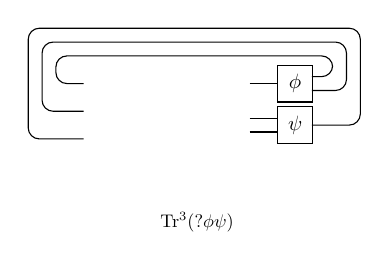
\begin{tikzpicture}[yscale=-1,x=1em,y=1em]

    \draw [rounded corners] (7,1.75) -- (8,1.75);
    \draw [rounded corners] (7,0) -- (8,0);
    \draw [rounded corners] (9.25,-0.25) -- (10,-0.25) -- (10,-1) -- (0,-1) -- (0,0) -- (1,0);
    \draw [rounded corners] (9.25,0.25) -- (10.5,0.25) -- (10.5,-1.5) -- (-0.5,-1.5) -- (-0.5,1) -- (1,1);
    \draw [rounded corners] (7,1.25) -- (8,1.25);
    \draw [rounded corners] (9.25,1.5) -- (11,1.5) -- (11, -2) -- (-1,-2) -- (-1,2) -- (1,2);

    \node [draw, minimum height = 1.25em, minimum width = 1.25em, anchor=west] at (8,0) {\scalebox{0.75}{$\phi$}};
    \node [draw, minimum height = 1.25em, minimum width = 1.25em, anchor=west] at (8,1.5) {\scalebox{0.75}{$\psi$}};

    \node [anchor=center] at (5.1,5) {\scalebox{0.66}{Tr$^3(? \seq \phi \tensor \psi)$}};

\end{tikzpicture}
\end{document}
